\chapter{Plasma power estimate}
\label{ch:temperature}
Direct application of plasma leads to deposition of accelerated particles on target. For non thermal blood coagulation it's fundamental that on biological tissues that a temperature increase due to this application must be below dangerous limits.

With the supposition that the main heating mechanism of our source is by convection, it is possible to estimate heat transfer rate, i.e. power, due to plasma application on a target. During this work only inorganic targets are utilized, while PCC will be applied to samples of blood and to living subjects, where heating effects are different if compared to inorganic matter. Heat transfer in living biological tissue is a complicated combination of thermal conduction, convection, perfusion of blood and metabolic heat generation \cite{ShitTemp}. The hypotesis behind the estimate of plasma power in this work is that the interaction between heat transfer mechanisms in biological tissues and heat deposition mechanism of our source is negligible. Under those conditions, with this power estimate will be possible to evaluate the temperature increase due to plasma application on every target once their thermal characteristics are know (for a review of thermal conduction parameters in biological tissues see \cite{biotissues}).
Even if the studied case is particular and has many limits, this analysis gives a rough estimate of plasma power dependencies from application parameters such as pulse repetition rate or distance between source and target.

\section{Experimental setup}
Plasma heat power is estimated measuring how much temperature increases with the application of plasma on a target with known heat capacity. The use of a thermocamera allows to study target's temperature profile in its entirety, visualizing also heat conduction on target's borders.
An object at thermal equilibrium in a temperature range around \SI{300}{\kelvin} emits radiation in the long-wavelength infrared region (from \num{8} to \SI{15}{\micro\meter}). This radiation can be collected and it's intensity measured by a bolometer, evaluating the temperature of the object from it's infrared emission, as in common thermal cameras (\cite{Gade2014}). The detector more used is an uncooled microbolometer VOx with an array of pixels as in figure \ref{fig:microbol}. Incident radiation strikes a material that has an absorption peak in infrared wavelenght, temperature increases changing the electrical resistance of the circuit and the resulting current intensity is measured and associated to collected radiation intensity.
\begin{figure}
 \centering
 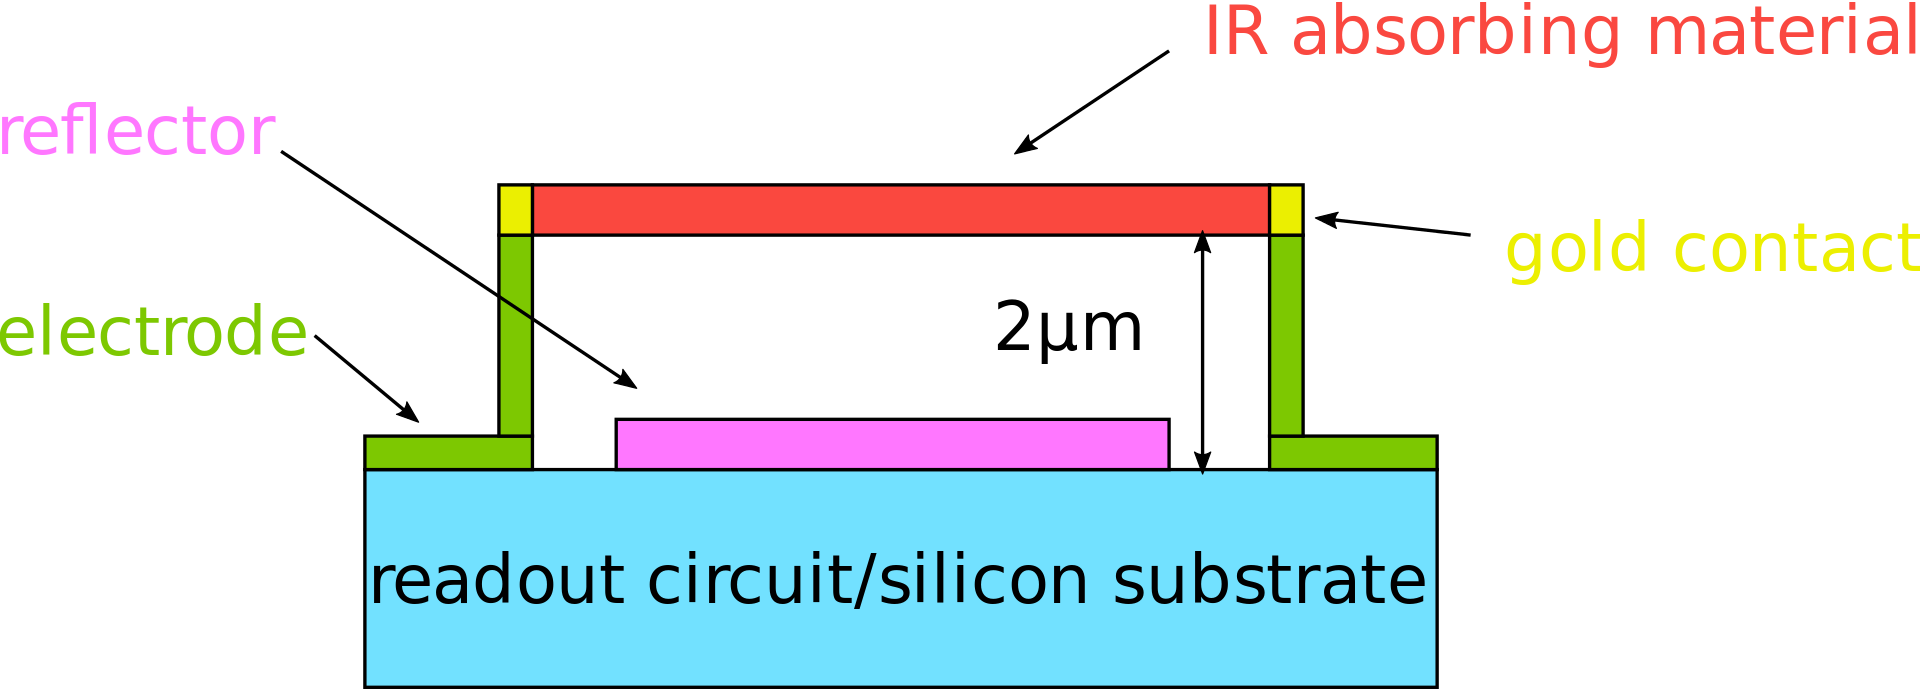
\includegraphics[width=0.4\textwidth]{Images/Temperature/Microbolometer.png}
 \caption{Rapresentation of pixel in a microbolometer detector. When incident radiation arrives on the pixel, temperature increases and electric resistance of the circuit changes, giving rise to a current intensity proportional to radiation intensity.}
 \label{fig:microbol}
\end{figure}


\paragraph{Camera}
The target is observed by a termographic camera \emph{FLIR A655sc} (\cite{flircamera}) with a spectral range of $\num{7.5}-\SI{14}{\micro\meter}$, resolution $\num{640}\times\num{480}$ and detector pitch \SI{17}{\micro\meter}, equipped with a lens with focal \SI{41.3}{\milli\meter} (field of view \ang{15}).
Temperature evolution is a phenomenon with charateristic time of several seconds, to have a reasonable resolution frame rate acquisition is set at \num{2} FPS.

The temperature conversion between intensity of the radiation and temperature is done by \emph{FLIR} software, setting the appropriate emissivity.

\paragraph{Source}
The source is the latest one, prototype \textbf{B} in chapter \ref{ch:electric}, at different pulse repetition frequencies $f$ and voltage peak values $V_p$. Plasma formation and deposition it's not a continuos phenomenon, it happens in correspondance of voltage pulses, with a charateristic time around \SI{1}{\micro\second}, see chapter \ref{ch:shape}. Given a time interval, $f$ defines the number of pulses that arrives in that interval.

The gas used to produce plasma is helium, with flow of \SI{2}{\liter/\minute}.

\paragraph{Target}
The target is an aluminium disk, with radius \SI{7}{\milli\meter} and height \SI{1}{\milli\meter}, on a plastic support with width \SI{5}{\milli\meter}.
Aluminium has specific heat capacity $c_p = \SI{897}{\joule/\kilogram\kelvin}$ and density $\rho = \SI{2700}{\kilogram/\meter^3}$, corresponding to target heat capacity $C = \SI{0.373(5)}{\joule/\kelvin}$.

Target is positioned at a distance of \SI{210}{\milli\meter} from camera lens. At those conditions, once the image is on focus, pixel to pixel distance on acquired frames is \SI{86.4}{\micro\meter}.

To verify relation between power and application distance the target is positioned at three distance values from the en of the source head: \num{5.5}, \num{7.5} or \SI{9.5}{\milli\meter}.

\paragraph{Measurements procedure}
Ultimately measurements are done with different voltage pulse repetition frequencies $f$, voltage peak values $V_p$ and distances between target and source $d$.
Once those parameters are set, the measure follows an approximative timeline:
\begin{itemize}
 \item acquisition of at least \num{4} frames for background evaluation in \SI{2}{\second}
 \item start of gas flow for a minimum of \SI{5}{\second}
 \item start of the discharge for a minimum of \SI{30}{\second}
 \item stop of the discharge and acquisition with only gas flow for \SI{5}{\second}
 \item stop of gas flow
\end{itemize}

Start and end time for those phases can be observed directly from measures.

\section{Temperature profile}
Every frame gives information on the temperature of every pixel of acquired image at a given time, as in figure \ref{fig:exframe}. To find the interested temperature difference, background temperature before discharge is evaluated as the average value acquired before gas opening and subtracted to pixel value in other frames. In a given direction the temperature profile is shown in figure \ref{fig:exframe}.
\begin{figure}
 \centering
 \subfloat[Frame $t = \SI{25}{\second}$.]{
    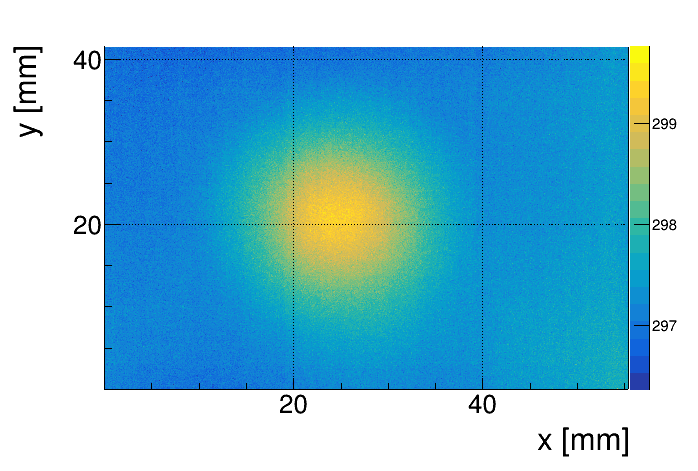
\includegraphics[width=0.48\textwidth]{Images/Temperature/f5t4d4_esframe_25s_2.png}
 }
 \hfill
 \subfloat[$\Delta T$ profile along x direction at $t = \SI{25}{\second}$]{
    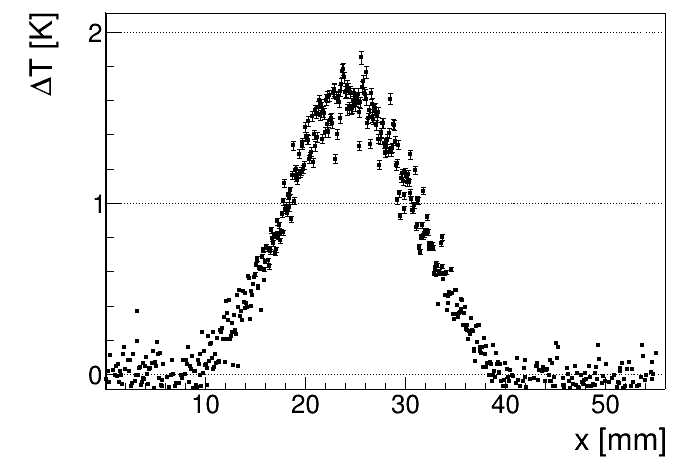
\includegraphics[width=0.48\textwidth]{Images/Temperature/f5t4d4_esprofilo_25s_2.png}
 }
 \caption{Example of measurement during discharge with parameters $f = \SI{5}{\kilo\hertz}$, $V_p = \SI{7.2}{\kilo\volt}$ and $d = \SI{5.5}{\milli\meter}$.}
 \label{fig:exframe}
\end{figure}


Source is pointed to target center, for frames acquired with the discharge can be seen clearly where the temperature rises and can be estimated the application position. A square window with edge \SI{15}{\milli\meter} si centered around the point with maximum temperature, to see the temperature increase on all the target. A gaussian interpolation inside the square allows to find the center position, compatible in each measurements set, at coordinates $x_{c} = \SI{25.06(20)}{\milli\meter}$, $y_{c} = \SI{21.17(20)}{\milli\meter}$.

It's interesting to note that when there is only gas flowing on the target, temperature increases radially from the center, in an area larger then the target area, while when there is plasma, temperature increases rapidly in an area compatible with the target dimensions. It's possible that gas before ionization creates a gas layer with a radius larger then the target radius, but considering temperature increase only around the target it doesn't gives problems in heat power evaluation due to discharge.

From each of those frames the average temperature difference and it's evolution are evaluated as shown in figure \ref{fig:Tavg}. This graph allows to extrapolate time intervals for gas flow and discharge: where temperature changes rapidly there is gas opening, source activation, discharge end and gas flow stop. In figure \ref{fig:dis_profiles} an example of how temperature profile changes during discharge.
\begin{figure}
 \centering
 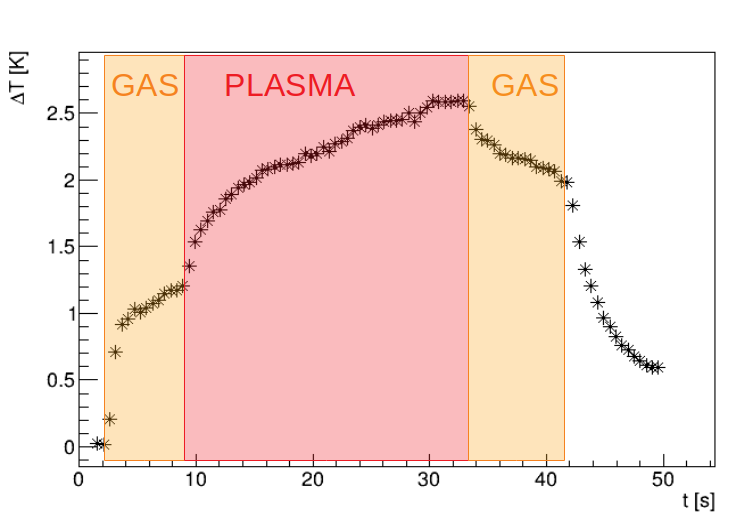
\includegraphics[width=0.6\textwidth]{Images/Temperature/f5t4d4_Tavg_lines.png}
 \caption{Average increase in temperature for every frame at different times, on a square around the target. There are three phases highlighted: gas phase before source activation, plasma phase and gas phase after source power off.}
 \label{fig:Tavg}
\end{figure}

\begin{figure}
 \centering
 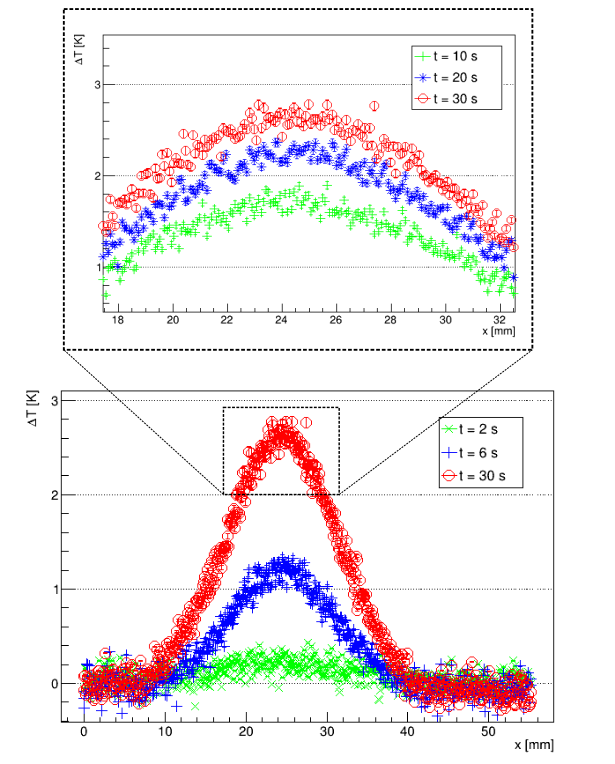
\includegraphics[width=0.6\textwidth]{Images/Temperature/f5t4d4_profilo_tempi_zoom.png}
 \caption{Evolution of temperature profile in x direction, with a zoom on the region around the target, for different times and phases: $t = \SI{2}{\second}$ before gas opening, $t = \SI{6}{\second}$ after gas opening and before discharge, $t = $\num{10}, \num{20}, \SI{30}{\second} during discharge. }
 \label{fig:dis_profiles}
\end{figure}


\section{Power estimation}
During the plasma phase, temperature increase in target can be defined as the sum of power deposition plus thermalization contributions (see \cite{Pimazzoni2018}), as in equation \ref{eq:dT}, where $m$ is the mass of the portion of target considered, $c_p$ is aluminium specific heat capacity, $P$ is power deposited by plasma on target, $T_{0}$ is a temperature limit and $k$ a costant parameter dependant from the target.
\begin{equation}
 m c_p \frac{dT}{dt} = P - k(T-T_{\text{lim}})
 \label{eq:dT}
\end{equation}

The anlytical result of this equation is an exponential function, as in figure \ref{fig:dTfit} for the center pixel in the image. The downside of the exponential fit it's that isn't possible to evaluate the contribution of power deposition from it. From temperature variation for temperatures close to $T_{0}$, where the thermalization contribute is neglectable, is possible to extrapolate parameter $P$ with a linear fit. The power parameter resulting from this interpolation is not a precise value because there are also thermalization contributes, but it is useful to study its behavior varying other parameters.
\begin{figure}
 \centering
 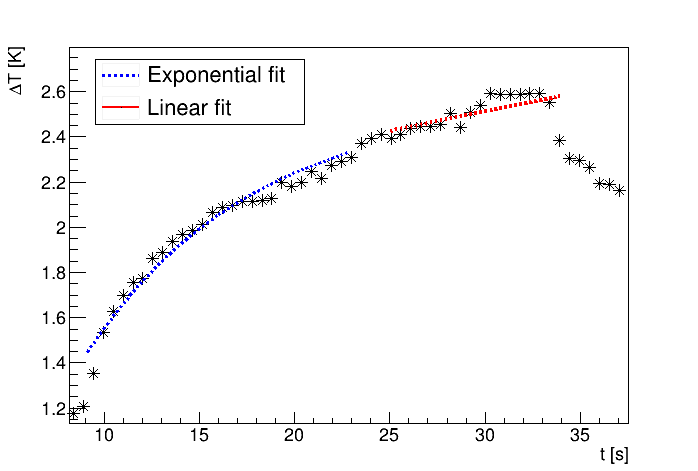
\includegraphics[width=0.6\textwidth]{Images/Temperature/f5t4d4_fits.png}
 \caption{Average increase of temperature for a restricted time ranges inside plasma phase, with exponential and linear interpolations. The exponential fit shows the analytical solution for equation \ref{eq:dT}, the linear fit is the one from wich power is extrapolated.}
 \label{fig:dTfit}
\end{figure}

To assure that temperature variation are observed only inside the target, only pixels within a radius of \SI{7}{\milli\meter} from the center of plasma application are considered. The maverage temperature variation in those conditions follows equation \ref{eq:dTpix}, where $\rho$ is aluminium density, $h$ is target width, $A_p$ is target area, $T_{\text{avg}}$ is the average temperature of a pixel, $T_p$ is the temperature of a pixel.
\begin{equation}
 m c_{p} T_{\text{avg}}(t) = \rho h A_{p}\frac{\sum_{\text{pixels}} T_{p}}{N_{\text{pixels}}} = P t + T_{0}
 \label{eq:dTpix}
\end{equation}


Plasma deposition isn't continuos in time but it happens within time intervals, as described in chapter \ref{ch:shape}.
Power evaluated considering the total time interval of plasma application is an effective power $P_{\text{eff}}$ that doesn't take into consideration the real time interval of interaction between plasma and target, a fraction of the total one. An estimate of the power associated with a single pulse $P_{\text{pulse}}$ can be found considering the time interval for the interaction of every pulse $\Delta t_{\text{pulse}}$ multiplied by the rate of pulses during the discharge $f$, as in equation \ref{eq:power}. An appropriate time pulse duration is $\Delta t_{\text{pulse}} = \SI{1}{\micro\second}$, as shown in chapter \ref{ch:shape}.
\begin{equation}
 P_{\text{pulse}} = \frac{P_{\text{eff}}}{\Delta t_{\text{pulse}} \, f}
 \label{eq:power}
\end{equation}


\paragraph{Pulse rate dependency}
Power parameter is evaluated with different pulse repetition rate, voltage peak value set at $V_{p} = \SI{7.2}{\kilo\volt}$ and distance between source and target $d = \SI{5.5}{\milli\meter}$. In figure \ref{fig:Pfr} there are effective power during the discharge and the pulse power relative to a single pulse. As expected the effective power is proportional to frequency of pulses: greater frequency means more pulses in a given time. It's instead intersting to note that power for a single pulse decreases with increasing pulse rate. 
An explanation could be that for different pulse repetition rate the time interval relative to the single pulse, i.e. the time interval during which we see plasma bullets, decreases from $\Delta t_{\text{pulse}} = \SI{1}{\micro\second}$ for $f = \SI{5}{\kilo\hertz}$ to values around $\Delta t_{\text{pulse}} = \SI{500}{\nano\second}$ for $f = \SI{25}{\kilo\hertz}$. This result could imply that for higher frequencies bullets have increasing speed.
\begin{figure}
 \centering
 \subfloat[Average power during discharge.]{
    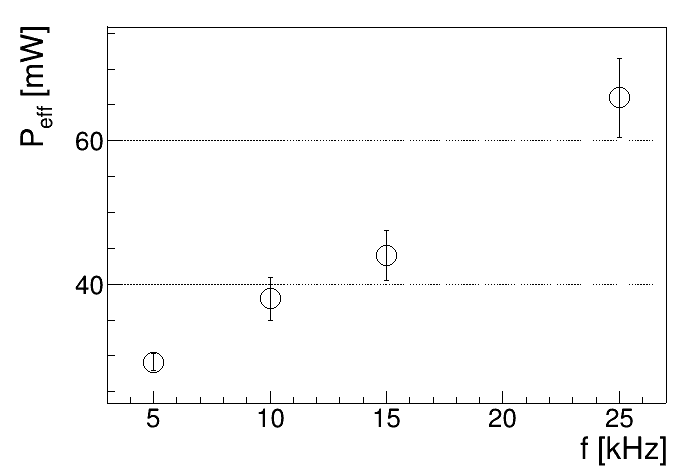
\includegraphics[width=0.48\textwidth]{Images/Temperature/Peff_fr_2.png}
 }
 \subfloat[Power relative to a single voltage pulse.]{
    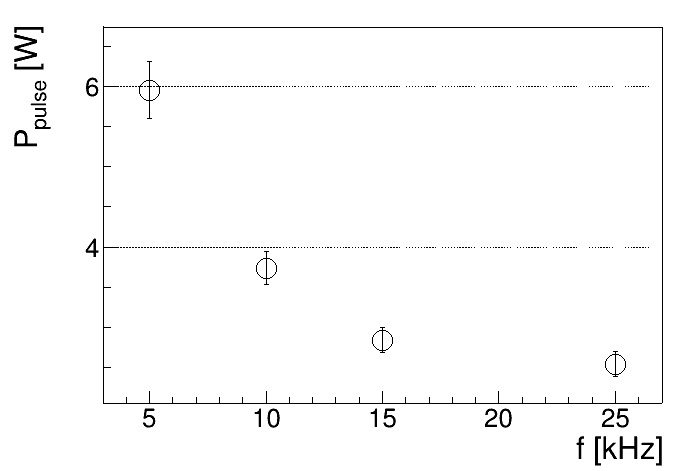
\includegraphics[width=0.48\textwidth]{Images/Temperature/Ppulse_fr_2.png}
 }
 \caption{Plasma power deposition on target for different pulse repetition rates.}
 \label{fig:Pfr}
\end{figure}


\paragraph{Voltage peak value dependency}
Temperature increase is observed with distance between source and target $d = \SI{5.5}{\milli\meter}$ and pulse repetition rate $f = \SI{5}{\kilo\hertz}$, for different voltage values. From figure \ref{fig:PVp} it is possible to see that power for the single pulse is correlated with the voltage peak value and increases rapidly when voltage increases. For voltage values from \SI{5.0}{\kilo\volt} to \SI{9.2}{\kilo\volt} temperature increase rate goes from \SI{7.8}{\milli\kelvin/\second} to \SI{85.2}{\milli\kelvin/\second}. With the higher voltage it is observed a temperature increase up to \SI{2.2}{\kelvin} in \SI{25}{\second} of plasma application. This behavior is expected because with an higher peak voltage value there is more electrical power transfered from the source and bullets have higher velocity, as described in chapter \ref{ch:shape}.
\begin{figure}
 \centering
 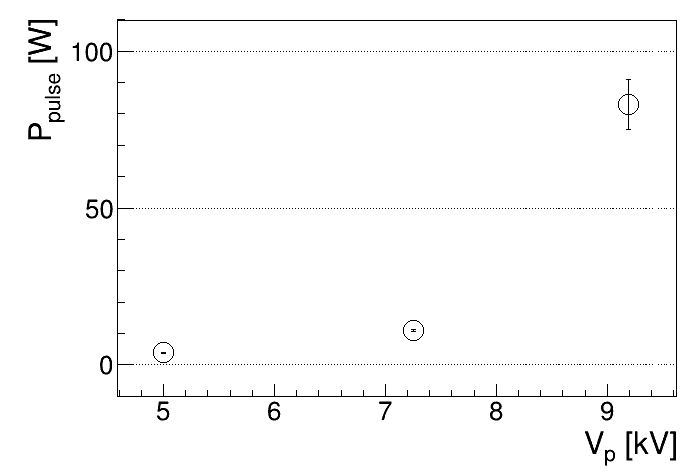
\includegraphics[width=0.6\textwidth]{Images/Temperature/Ppulse_Vp_2.png}
 \caption{Plasma power of a single pulse for different voltage peak values.}
 \label{fig:PVp}
\end{figure}

\paragraph{Distance dependency}
The influence of the distance between target and source is measured setting voltage peak at $V_{p} = \SI{7.2}{\kilo\volt}$ and $f = \SI{5}{\kilo\hertz}$. In figure \ref{fig:Pd} it is possible to see how power decreases with incresing distance, as expected because for higher distances between source and target, bullets lose more energy before the impact and will transfer less energy to the target. For distance going from \SI{5.5}{\milli\meter} to \SI{7.5}{\milli\meter} the pulse power loss rate is of \SI{0.28(5)}{\watt/\milli\meter}.
\begin{figure}
 \centering
 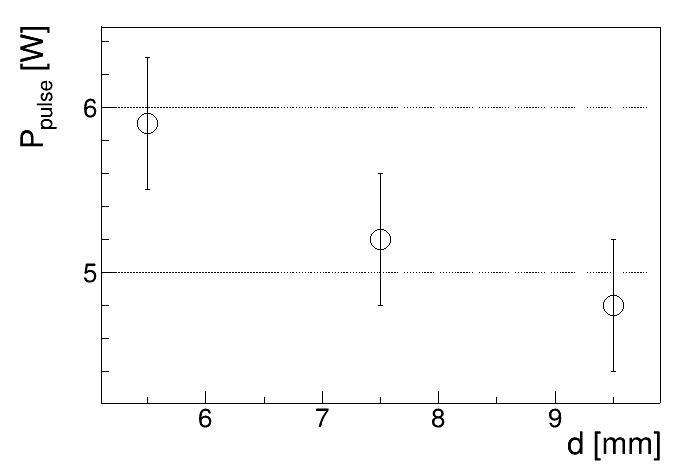
\includegraphics[width=0.6\textwidth]{Images/Temperature/Ppulse_d_2.png}
 \caption{Plasma power of a single pulse for different target distances.}
 \label{fig:Pd}
\end{figure}
